%!TEX root = ../main.tex
\subsection{Normalverteilung}
Die Normalverteilung wird Verwendet bei Merkmalen,
\begin{itemize}
	\item die stetig oder quasi-stetig sind,
	\item deren Daten um einen Mittelwert streuen,
	\item deren Daten seltener werden, je größer der Abstand zum Mittelwert.
\end{itemize}

Eine Zufallsvariable $X$ ist \emph{normalverteilt} mit Paramtern $\mu$ und $\sigma^2$, wenn für ihre Dichte gilt
\begin{center}
	\begin{tikzpicture}[scale=0.9]
		\draw[->, line width=0.3mm] (0,6) to (8.5,6) node[below] {$x$};
		\draw[->, line width=0.3mm] (0,6) to (0,11) node[right] {$f^X(x)$};
		\draw[->, line width=0.3mm] (0,0) to (8.5,0) node[below] {$x$};
		\draw[->, line width=0.3mm] (0,0) to (0,5) node[right] {$F^X(x)$};

		\draw[line width=0.5mm,scale=1,domain=0:8,smooth,variable=\x,blue] plot ({\x},{4*exp(-(\x-4)*(\x-4)/2.7)+6.05});


		\draw[line width=0.5mm,scale=1,domain=0:4,smooth,variable=\x,blue] plot ({\x},{2*exp((\x-4)/1.3)});
		\draw[line width=0.5mm,scale=1,domain=4:8,smooth,variable=\x,blue] plot ({\x},{-2*exp(-(\x-4)/1.3)+4});



		\draw (4,2) node (Fmu) [fill = white,circle,inner sep = 0pt,minimum size = 4pt,draw] {};
		\draw (4,10.04) node (fmu) [fill = white,circle,inner sep = 0pt,minimum size = 4pt,draw] {};

		\draw (5.3,8.2) node (fmu+) [fill = white,circle,inner sep = 0pt,minimum size = 4pt,draw] {};
		\draw (2.7,8.2) node (fmu-) [fill = white,circle,inner sep = 0pt,minimum size = 4pt,draw] {};

		\draw (5.3,6) node (muf+) [rectangle,inner sep = 0pt,minimum size = 0pt,minimum height=4pt,draw, label={below:$\mu+\sigma$}] {};
		\draw (2.7,6) node (muf-) [rectangle,inner sep = 0pt,minimum size = 0pt,minimum height=4pt,draw, label={below:$\mu-\sigma$}] {};

		

		\draw (4,6) node (muf) [rectangle,inner sep = 0pt,minimum size = 0pt,minimum height=4pt,draw, label={below:$\mu$}] {};
		\draw (4,0) node (muF) [rectangle,inner sep = 0pt,minimum size = 0pt,minimum height=4pt,draw, label={below:$\mu$}] {};

		
		\draw (0,0) node (null) [rectangle,inner sep = 0pt,minimum size = 0pt,minimum width=4pt,draw, label={left:$0$}] {};
		\draw (0,4) node (eins) [rectangle,inner sep = 0pt,minimum size = 0pt,minimum width=4pt,draw, label={left:$1$}] {};
		\draw (0,2) node (einhalb) [rectangle,inner sep = 0pt,minimum size = 0pt,minimum width=4pt,draw, label={left:$\frac12$}] {};
		\draw[dotted, gray] (eins) -- (8, 4);


		\draw[red, line width=0.3mm, dashed] (muF) -- (Fmu) -- (einhalb);
		\draw[red, line width=0.3mm, dashed] (muf) -- (fmu);
		
		\draw[green, line width=0.3mm, dashed] (fmu+) -- (muf+);
		\draw[green, line width=0.3mm, dashed] (fmu-) -- (muf-);
			

		\draw (-4, 8.5) node {$\displaystyle f^X(x)=\frac{1}{\sqrt{2\pi\sigma^2}}*\exp\left(\frac{-(x-\mu)^2}{2\sigma^2}\right)$};
	\end{tikzpicture}	
\end{center}
Wir schreiben dann $X\sim\norm(\mu,\sigma^2)$.
\paragraph{Eigenschaften:}
\begin{itemize}
	\item $f$ ist symmetrisch zum Mittelwert $\mu$.
	\item Der Erwartungswert von $X$ ist der Mittelwert, d.h. $E(X)=\mu$. Die Lage der Dichtefunktion wird durch $\mu$ bestimmt.
	\item Für die Dichtefunktion gilt $\int_{-\infty}^{\infty} f^X(t)\intd t = 1$.
	\item Für die Varianz gilt $V(X)=\sigma^2$. Der zweite Parameter der Normalverteilung gibt also die Breite der Dichtefunktion an.
	\item Die Dichtefunktion hat ihre Wendepunkte bei $\mu\pm\sigma$.
	\item Die Verteilung $F^X(x)=\int_{-\infty}^{x} f^X(t)\intd t$ hat keine geschlossene Form und ist daher teuer/ aufwändig zu berechnen. Man verwendet daher oft die \emph{Standardnormalverteilung} um Werte zu berechnen.
	\item {\bf Transformiert} man eine normalverteilte Zufallsvariable $X\sim\norm(\mu,\sigma^2)$, zu $Y=aX+b$, dann ist $Y$ wiederum normalverteilt mit $Y\sim\norm(a\mu+b, a^2\sigma^2)$.
	\item Für zwei \emph{unabhängige} Zufallsvariablen $X\sim\norm(\mu_x,\sigma_x^2)$ und $ Y\sim\norm(\mu_y,\sigma_y^2)$ ist die {\bf Summe} der beiden wieder normalverteilt, $(X+Y)\sim\norm(\mu_x+\mu_y,\sigma_x+\sigma_y)$.
\end{itemize}

\subsubsection{Standardnormalverteilung}
Eine Zufallsvariable $Z$ ist Standard-normalverteilt, wenn $Z\sim\norm(0,1)$.
Ihre Dichte ist dann gegeben als
\begin{equation*}
	\varphi(x)=\frac{1}{\sqrt{2\pi}}*e^{-\frac12x^2}
\end{equation*}

Dann ist $E(Z)=0$ und $V(Z)=1$. Eine allgemeine normalverteilte Zufallsvariable $X\sim\norm(\mu,\sigma)$ lässt sich damit einfach wie folgt auf $Z$ reduzieren
\begin{equation*}
	X\sim\norm(\mu, \sigma)\Rightarrow Z:\frac{X-\mu}{\sigma}\sim\norm{0,1}
\end{equation*}
Damit folgt dann
\begin{enumerate}
	\item Tabellieren von $\Phi(x)=\int_{-\infty}^x \varphi(t)\intd t$ reicht aus um die Verteilungsfunktion einer beliebig parametrisierten Normalverteilung zu berechnen.
	\begin{align*}
		F^X(X)&=P(X\leq x)\\
		&=P\left(\frac{X-\mu}{\sigma}\leq \frac{x-\mu}{\sigma}\right)\\
		&=P\left(Z\leq\frac{x-\mu}{\sigma}\right)\\
		&=\Phi\left(\frac{x-\mu}{\sigma}\right)
	\end{align*}
	\item Analog ist $X=\mu+\sigma Z$, damit sind dann Varianz und Erwartungswert
	\begin{align*}
		E(X)&=E(\mu+\sigma Z)=\mu\\
		V(X)&=V(\mu+\sigma Z)=\sigma^2
	\end{align*}
\end{enumerate}



\subsubsection{Quantile der Normalverteilung}
Die Quantile von Verteilungen können immer über die inverse Verteilungsfunktion berechnet werden. Das heißt für die (Standard-) Normalverteilung ist $z_p$ das $p$-Quantil, wenn $\Phi(z_p)=p$ ist ($0<p<1$).
\begin{center}
	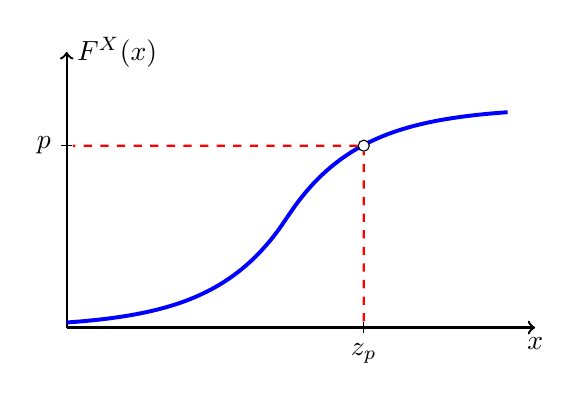
\begin{tikzpicture}[scale=0.7]
		\draw[->, line width=0.3mm] (0,0) to (8.5,0) node[below] {$x$};
		\draw[->, line width=0.3mm] (0,0) to (0,5) node[right] {$F^X(x)$};

		\draw[line width=0.5mm,scale=1,domain=0:4,smooth,variable=\x,blue] plot ({\x},{2*exp((\x-4)/1.3)});
		\draw[line width=0.5mm,scale=1,domain=4:8,smooth,variable=\x,blue] plot ({\x},{-2*exp(-(\x-4)/1.3)+4});

		\draw (5.39,3.3) node (fp) [fill = white,circle,inner sep = 0pt,minimum size = 4pt,draw] {};
		
		\draw (5.39,0) node (zp) [rectangle,inner sep = 0pt,minimum size = 0pt,minimum height=4pt,draw, label={below:$z_p$}] {};	
	
		\draw (0,3.3) node (p) [rectangle,inner sep = 0pt,minimum size = 0pt,minimum width=4pt,draw, label={left:$p$}] {};

		\draw[red, line width=0.3mm, dashed] (zp) -- (fp) -- (p);

	\end{tikzpicture}	
\end{center}
Diese Berechnungen lassen sich ebenso transformieren um Quantile für Normalverteilungen mit allgemeinen Parametern zu berechnen.

In der Abbildung unten ist das $p$-Quantil und das $(1-p)$-Quantil in die Dichtefunktion eingezeichnet, die grünen Flächen entsprechen jeweils der Wahrscheinlichkeit $1-p$.
\begin{center}
	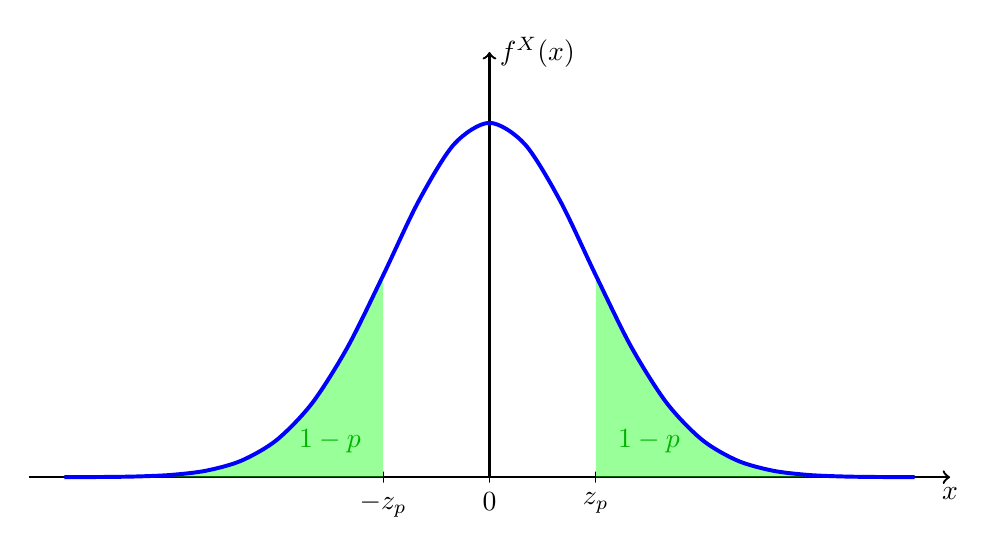
\begin{tikzpicture}[scale=0.9]
		\draw[->, line width=0.3mm] (-6.5,0) to (6.5,0) node[below] {$x$};
		\draw[->, line width=0.3mm] (0,0) to (0,6) node[right] {$f^X(x)$};

		\filldraw[scale=1,domain=-6:-1.5,smooth,variable=\x,fill=green, opacity=0.4, draw=none] plot ({\x},{5*exp(-\x*\x/4)}) -- (-1.5,0);
		\filldraw[scale=1,domain=1.5:6,smooth,variable=\x,fill=green, opacity=0.4, draw=none] plot ({\x},{5*exp(-\x*\x/4)}) -- (1.5,0);
		
		\draw[line width=0.5mm,scale=1,domain=-6:6,smooth,variable=\x,blue] plot ({\x},{5*exp(-\x*\x/4)});

		\draw (1.5,0) node (zp) [rectangle,inner sep = 0pt,minimum size = 0pt,minimum height=4pt,draw, label={below:$z_p$}] {};
		\draw (-1.5,0) node (-zp) [rectangle,inner sep = 0pt,minimum size = 0pt,minimum height=4pt,draw, label={below:$-z_p$}] {};

		\draw (-2.25,0.5) node[green!70!black] {$1-p$};
		\draw (2.25,0.5) node[green!70!black] {$1-p$};
		
		\draw (0,0) node (null) [rectangle,inner sep = 0pt,minimum size = 0pt,minimum height=4pt,draw, label={below:$0$}] {};
		
	\end{tikzpicture}	
\end{center}
Davon ausgehend erhält man die sogenannten zentralen Schwankungsbereiche, auch Sigma-Bereiche.
Diese sind für $X\sim\norm(\mu,\sigma^2)$ die Intervalle
\begin{equation*}
	\mu-k*\sigma\leq X\leq \mu+k*\sigma\quad k\in\simpleset{1,2,\ldots}
\end{equation*}

In der unten stehenden Abbildung sind rechts vom Mittelwert die ersten drei (halben) Sigma-Bereiche eingezeichnet, diese erweitern sich symmetrisch auf die linke Seite. Die Flächen stehen für die Wahrscheinlichkeit, dass die Zufallsvariable $X$ Werte im $x$-Abschnitt der Fläche annimmt.
\begin{center}
	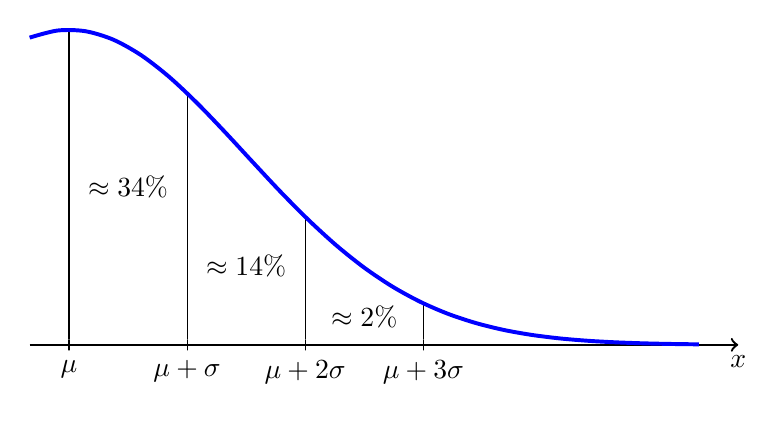
\begin{tikzpicture}
		\draw[->, line width=0.3mm] (-0.5,0) to (8.5,0) node[below] {$x$};
		
		\draw (0,0) node (mu) [rectangle,inner sep = 0pt,minimum size = 0pt,minimum height=4pt,draw, label={below:$\mu$}] {};
		\draw (1.5,0) node (mu1) [rectangle,inner sep = 0pt,minimum size = 0pt,minimum height=4pt,draw, label={below:$\mu+\sigma$}] {};
		\draw (3,0) node (mu2) [rectangle,inner sep = 0pt,minimum size = 0pt,minimum height=4pt,draw, label={below:$\mu+2\sigma$}] {};
		\draw (4.5,0) node (mu3) [rectangle,inner sep = 0pt,minimum size = 0pt,minimum height=4pt,draw, label={below:$\mu+3\sigma$}] {};

		\draw (mu) -- (0,4);
		\draw (mu1) -- (1.5,3.2);
		\draw (mu2) -- (3,1.6);
		\draw (mu3) -- (4.5,0.51);

		\draw[line width=0.5mm,scale=1,domain=-0.5:8,smooth,variable=\x,blue] plot ({\x},{4*exp(-\x*\x/10)});

		\draw (0.75,2) node {$\approx 34\%$};
		\draw (2.25,1) node {$\approx 14\%$};	
		\draw (3.75,0.35) node {$\approx 2\%$};			
	\end{tikzpicture}	
\end{center}
Es ergeben sich damit also die Wahrscheinlichkeiten
\begin{itemize}
	\item $P(\mu-\sigma\leq X\leq \mu+\sigma)=68\%$
	\item $P(\mu-2\sigma\leq X\leq \mu+2\sigma)=95.5\%$
	\item $P(\mu-3\sigma\leq X\leq \mu+3\sigma)=99.7\%$
\end{itemize}




